\documentclass[a4paper, 12pt]{extreport}
\usepackage[margin=1in]{geometry}
\usepackage{tikz}
\usetikzlibrary{calc, shapes.geometric, arrows.meta, positioning}
\usepackage{setspace}
\graphicspath{ {../../resources/images/} }
\usepackage[titles]{tocloft}
\usepackage{titlesec}
\usepackage[hidelinks]{hyperref}
\usepackage{pdfpages}
\titleformat{\chapter}[hang]{\huge\bfseries}{\thechapter}{20pt}{\vspace{0.5em}}
\titlespacing*{\chapter}{0pt}{-3em}{1.1\parskip}
\usepackage[backend=biber, style=ieee]{biblatex}
\usepackage{parskip}
\setlength{\parindent}{1cm}
\setlength{\parskip}{.5\baselineskip}
\usepackage[nottoc,numbib]{tocbibind}
\addbibresource{../../resources/citation.bib}
%\usepackage{tabularx}
\usepackage{tabularray}
\usepackage{multirow}
\usepackage{amsmath,amssymb}
\usepackage{adjustbox}
\usepackage[T1]{fontenc}
\usepackage[final]{microtype}
\usepackage{subcaption}
\usepackage[bottom]{footmisc}
\usepackage{pgfgantt}
\usepackage{pdflscape}


\begin{document}
	
	% defining pieces for figures
	\def\opiece{\tikz{\draw[fill=yellow](0,0) rectangle (2,2);}}
	\def\ipiece{\tikz{\draw[fill=cyan](0,0) rectangle (4,1);}}
	\def\tpiece{\tikz{\draw[fill=violet](0,0) -- (3,0) -- (3,1) -- (2,1) -- (2,2) -- (1,2) -- (1,1) -- (0, 1) -- cycle;}}
	\def\zpiece{\tikz{\draw[fill=red](0,1) -- (1,1) -- (1,0) -- (3,0) -- (3,1) -- (2,1) -- (2,2) -- (0,2) -- cycle;}}
	\def\spiece{\tikz{\draw[fill=green](0,0) -- (2,0) -- (2,1) -- (3,1) -- (3,2) -- (1,2) -- (1,1) -- (0,1) -- cycle;}}
	\def\jpiece{\tikz{\draw[fill=blue](0,0) -- (3,0) -- (3,1) -- (1,1) -- (1,2) -- (0,2) -- cycle;}}
	\def\lpiece{\tikz{\draw[fill=orange](0,0) -- (3,0) -- (3,2) -- (2,2) -- (2,1) -- (0,1) -- cycle;}}
	\def\garbage#1#2{\tikz{\draw[fill=black!40!white](0,0) -- (0,#1) -- (#2-1,#1) -- (#2-1,0) -- cycle; \draw[fill=black!40!white](#2, 0) -- (10,0) -- (10,#1) -- (#2,#1) -- cycle}}

	\onehalfspacing
	
	\begin{titlepage}
		
		\centering
		\begin{tikzpicture}
			\node[] at (current page.north west){%
				
\includegraphics[height=3.5cm]{logos/sunway-set}};
		\end{tikzpicture}
		
		\vspace{.5cm}
		
		\begin{center}
			\textbf{\large CAPSTONE PROJECT 1} \\
			\textbf{\large Planning Document} \\
			\vspace{1cm}
			\textbf{\large Playing Versus Tetris with Nature-inspired Optimisation Algorithms}
			
			\vspace{1cm}
			
			by
			
			\vspace{1cm}
			
			\large Yap Wei Xiang \\
			21067939
			
			\vspace{1cm}
			
			Bachelor of Science (Honours) in Computer Science
			
			\vspace{1cm}
			
			\large Supervisor: Dr Richard Wong Teck Ken
			
			\vspace{1cm}
			
			\normalsize Semester: April 2024 \\
			Date: 1 August 2024
			
			\vfill
			
			Department of Computing and Information Systems\\
			School of Engineering and Technology\\
			Sunway University
		\end{center}
		
	\end{titlepage}
	
	\pagenumbering{roman} % switch to roman numerals
	
	\chapter*{Abstract}
	
	\addcontentsline{toc}{chapter}{Abstract}
	
	\tableofcontents
	
	\listoftables
	
	\listoffigures
	
	\chapter{Introduction}
	
		\pagenumbering{arabic}
		
		% What is Tetris		
		Tetris is a popular video game created in 1984 by computer programmer Alexey Pajitnov  \cite{about-tetris}. It is a puzzle game that requires players to strategically place sequences of pieces known as "Tetriminos" into a rectangular Matrix (refer to Figure \ref{fig:tetrisgame}). In the classic game, players attempt to clear as many lines as possible by completely filling horizontal rows of blocks, but if the Tetriminos surpass the top of the Matrix, the game ends.
		
		\begin{figure}[h]
			\centering
				\begin{tikzpicture}[every node/.style={inner sep=-0.4pt,anchor=south west,scale=.4},scale=.4]
					\coordinate (sw) at (5,0);
					\coordinate (nw) at (5,20);
					\coordinate (se) at (15,0);
					\coordinate (ne) at (15,20);
					\draw[fill=black!10!white] (sw) -- (nw) -- (ne) -- (se) -- cycle;
					\node at ($(nw) - (4,5)$){\spiece};	
					\node at (sw){\ipiece};
					\node at ($(sw) + (4,0)$){\opiece};
					\node at ($(sw) + (2,1)$){\spiece};
					\node at ($(sw) + (1,1)$){\rotatebox{90}{\zpiece}};
					\node at ($(sw) + (0,1)$){\rotatebox{-90}{\jpiece}};
					\node at ($(sw) + (6,0)$){\tpiece};
					\node at ($(sw) + (7,1)$){\rotatebox{90}{\lpiece}};
					\node at ($(sw) + (5,1)$){\rotatebox{180}{\tpiece}};
					\node at ($(sw) + (2,3)$){\zpiece};
					\node at ($(sw) + (5,3)$){\opiece};
					\node at ($(se) - (1,-5)$){\rotatebox{90}{\ipiece}};
					\node at ($(ne) + (1,-2)$){\lpiece};
					\node at ($(ne) + (1,-5)$){\jpiece};
					\node at ($(ne) + (1,-8)$){\opiece};
					\node at ($(ne) + (1,-11)$){\ipiece};
					\node at ($(ne) + (1,-14)$){\tpiece};
					\draw[ultra thick] (sw) -- (nw) -- (ne) -- (se) -- cycle;
				\end{tikzpicture}
			\caption{\centering A typical modern Tetris game where four lines are about to be cleared. The Tetrimino on the left of the matrix is the \textit{Hold} piece and the pieces to the right of the matrix are collectively known as the \textit{Queue}.}
			\label{fig:tetrisgame}
		\end{figure}
		
		% Tetris and computer science
		Since its release, mathematicians and computer scientists have been intrigued by the game of Tetris, leading to a diverse array of research endeavours exploring the various facets of the game, including its computational complexity \cite{tetris-is-hard-even-to-approx}, and its possibility of being won \cite{can-you-win-at-tetris} \cite{how-to-lose-at-tetris}.
		
		\section{Motivation}
		
			% In this section, you'll explain why your capstone project is important and relevant. What inspired you to pursue this topic? Is there a particular problem or challenge in the field that you're interested in addressing?
			% Consider discussing the broader significance of your research topic, such as its potential impact on society, industry, or academia. Why should readers care about your project?
			% You might also highlight any personal or professional experiences that motivated your interest in the topic.
	 		
	 		In their paper, \citeauthor{tetris-is-hard-even-to-approx} showed that it is NP-complete to optimise several natural objective functions of Tetris \cite{tetris-is-hard-even-to-approx}. NP-completeness poses a significant challenge in computational problem-solving, as it denotes the absence of polynomial-time algorithms for efficient solutions \cite{sipser-intro-to-computation}. Moreover, the discovery of a polynomial-time algorithm for any NP-complete problem implies that any problem in the set of NP, encompassing efficiently verifiable but potentially difficult problems, could be solved in polynomial time \cite{sipser-intro-to-computation}. NP-completeness extends beyond Tetris, with real-life instances of NP-complete arising in diverse fields such as route optimisation \cite{route-optimisation-np-complete}, job scheduling \cite{job-scheduling-np-complete}, and medicine \cite{medical-diagnosis-np-complete}.
	 		
	 		To address these challenges, researchers have explored alternative approaches to tackle NP-complete problems, including the use of nature-inspired algorithms \cite{job-shop-ga}. Although they might fail at finding optimal solutions, nature-inspired algorithms are able to return acceptable solutions in shorter running times \cite{review-nia-wael}. In the context of optimising Tetris gameplay, studies have shown the effectiveness of using nature-inspired algorithms in playing the classic single-player game \cite{tetris-ga-lewis} \cite{swarm-tetris}. However, there remains limited research on the effectiveness of nature-inspired optimisation algorithms in the multiplayer versus variant of the game.
			
		\section{Problem Statement}
			
			% Here, you'll clearly define the problem or issue that your capstone project aims to address. What specific challenge or question are you seeking to answer?
			% Describe the current state of the problem and any existing solutions or approaches. What limitations or shortcomings do these solutions have?
			% Be concise and specific in articulating the problem statement, making it clear to readers what your project seeks to contribute to the field.
			
			% Despite the extensive research on classic Tetris, there is a significant gap in the literature regarding its multiplayer versus variant (refer to Figure \ref{tetrio}). This gap presents an intriguing problem within the field of computational gaming, as understanding the optimal strategies, challenges, and computational complexities unique to multiplayer versus Tetris remains largely uncharted territory.
			
			\textit{Versus Tetris} (refer to Figure \ref{fig:versus-example}) presents a unique challenge in computational gaming due to its complex dynamics and real-time competitive nature. While previous research regarding the use of nature-inspired algorithms for Tetris optimisation have focused on single-player scenarios, the effectiveness of these algorithms in the multiplayer context remains largely unexplored. Despite the demonstrated success of these algorithms in improving single-player Tetris gameplay, their application to the multiplayer variant poses distinct challenges due to a different rule set and differing objectives that require further investigation.
			
			\begin{figure}
					\begin{minipage}{.4\textwidth}
					\begin{tikzpicture}[every node/.style={inner sep=-0.4pt,anchor=south west,scale=.3},scale=.3]
						\coordinate (sw) at (5,0);
						\coordinate (nw) at (5,20);
						\coordinate (se) at (15,0);
						\coordinate (ne) at (15,20);
						\coordinate (gar) at (5,6);
						\draw[fill=black!10!white] (sw) -- (nw) -- (ne) -- (se) -- cycle;
						\node at ($(nw) - (3,5)$){\opiece};	
						\node at (sw){\garbage{2}{3}};
						\node at ($(sw) + (0,2)$){\garbage{4}{10}};
						\node at (gar){\jpiece};
						\node at ($(gar) + (3,0)$){\lpiece};
						\node at ($(gar) + (6,0)$){\opiece};
						\node at ($(gar) + (9,3)$){\rotatebox{90}{\ipiece}};
						\node at ($(ne) + (1,-2)$){\spiece};
						\node at ($(ne) + (1,-5)$){\zpiece};
						\node at ($(ne) + (1,-8)$){\tpiece};
						\node at ($(ne) + (1,-11)$){\ipiece};
						\node at ($(ne) + (1,-14)$){\tpiece};
						\draw[ultra thick] (sw) -- (nw) -- (ne) -- (se) -- cycle;
					\end{tikzpicture}
				\end{minipage} \hspace{3cm}
				\begin{minipage}{.4\textwidth}
					\begin{tikzpicture}[every node/.style={inner sep=-0.4pt,anchor=south west,scale=.3},scale=.3]
						\coordinate (sw) at (5,0);
						\coordinate (nw) at (5,20);
						\coordinate (se) at (15,0);
						\coordinate (ne) at (15,20);
						\draw[fill=black!10!white] (sw) -- (nw) -- (ne) -- (se) -- cycle;
						\node at ($(nw) - (4,5)$){\jpiece};	% HOLD
						\node at (sw){\rotatebox{-90}{\lpiece}}; 
						\node at ($(sw) + (3,0)$){\ipiece};
						\node at ($(sw) + (3,1)$){\zpiece};
						\node at ($(sw) + (6,0)$){\rotatebox{90}{\spiece}};
						\node at ($(sw) + (8,0)$){\opiece};
						\node at ($(nw) + (1,-13)$){\rotatebox{90}{\tpiece}};
						\node at ($(ne) + (1,-2)$){\ipiece}; % LOOKAHEAD
						\node at ($(ne) + (1,-5)$){\tpiece};
						\node at ($(ne) + (1,-8)$){\lpiece};
						\node at ($(ne) + (1,-11)$){\jpiece};
						\node at ($(ne) + (1,-14)$){\spiece};
						\draw[ultra thick] (sw) -- (nw) -- (ne) -- (se) -- cycle;
					\end{tikzpicture}
				\end{minipage}
				\caption{\centering A typical game of Versus Tetris. Both players are trying to send lines to each other. The grey blocks are \textit{Garbage Lines} sent from Player 2 (right) to Player 1 (left).}
				\label{fig:versus-example}
			\end{figure}
		
		\section{Aim}
		
			% The aim of your project is its overarching goal or objective. What do you hope to achieve through your research?
			% Summarize the main purpose of your project in a single sentence or paragraph. This should provide a clear, concise statement of what you intend to accomplish.
			% Your aim should align closely with the problem statement and reflect the broader motivation for your research.
			
			The aim of this capstone project is to assess the effectiveness of nature-inspired optimisation algorithms in playing the game of Versus Tetris. By integrating insights from nature-inspired algorithms, the project seeks to create a robust and adaptable Tetris-playing software capable of competing against human players or other Tetris-playing programs. Through this endeavour, the project aims to contribute valuable insights into the application of nature-inspired algorithms in addressing computationally complex problems.
		
		\section{Objectives}
		
			% Objectives are specific, measurable outcomes that you aim to achieve in order to fulfill your project's aim.
			% List the key objectives of your project, breaking them down into actionable steps or milestones. These objectives should directly address the problem statement and contribute to achieving the project's aim.
			% Consider using the SMART criteria (Specific, Measurable, Achievable, Relevant, Time-bound) to ensure that your objectives are well-defined and achievable within the scope of your project.
			
			The objectives of this project are as follows:
			
			\begin{enumerate}
				\item Formulate the problem of Versus Tetris for game AI.
				\item Develop a playable game of Tetris that simulates gameplay for training and emulation.
				\item Evaluate suitability of different nature-inspired optimisation algorithms to optimise gameplay strategies in Versus Tetris.
			\end{enumerate}
		
		\section{Project Scope}
			
			% Define the boundaries and focus areas of your capstone project in terms of its scope. What aspects of the problem will you address, and what will you exclude?
			% Discuss any limitations or constraints that may impact the scope of your project, such as time, resources, or access to data.
			% Clarify what readers can expect to find within the scope of your project and what may fall outside its boundaries.
			
			This project will focus specifically on the evaluation of nature-inspired optimisation algorithms in the context of multiplayer versus Tetris. It will entail the development of a playable Tetris game capable of simulating gameplay and the training of algorithms. This simulation environment will facilitate in the analysis and evaluation of these algorithms' performances. The scope includes the exploring of a range of nature-inspired algorithms to address the unique challenges inherent in Versus Tetris.
			
		
		% Exceptional overview of the proposed project.
		% The problem statement, objectives, scope of work, methodology, proposed outcome and timeline are written in a clear precise manner and presented in proper order.
	
	\chapter{Literature Review}
		
		% A well-articulated introduction that provides a clear, logical, and succinct description of content, scope, and organization of the review which draws the reader's attention to a central concern, debate or contention.
		% Body of section includes citations to a range of reliable sources that critically substantiate and contextualizes all major claims made.
		% Exceptional discussion that summarizes the body of review, highlights the most important findings (in your opinion) and its implication to the direction of the project.
		% Section is very well organized.
		% The review has clarity, simplicity, parsimony, which includes clear transitions and systematic use of headings and subheadings.
		
		% Background information: versus and regular tetris, differences, similarities, randomness
		% Justify why the literature review is about Tetris and not Versus Tetris
		
		Tetris, a timeless puzzle game created by Alexey Pajitnov in 1984, has captivated players and researchers alike with its engaging gameplay and complex strategic elements. The game challenges players to manipulate sequences of geometric shapes known as "Tetriminos" to clear horizontal lines within a confined space. Despite its simple premise, Tetris has inspired extensive research in computational complexity and artificial intelligence due to its inherent difficulty.
		
		This review will cover the fundamental challenges of Tetris, explore existing approaches, and assess the potential of nature-inspired algorithms to enhance gameplay strategies.	
				
		\section{The Difficulty of Tetris} \label{sec:diff-of-tetris}
		
			In their article, \citeauthor{tetris-is-hard-even-to-approx} \cite{tetris-is-hard-even-to-approx} proved that optimising several natural objectives of Tetris is NP-complete, even with a deterministic finite piece sequence. A deterministic finite piece sequence refers to a game at which the player knows every single piece in the sequence, and where there are finite pieces in the sequence, i.e. the game can end without the player losing. The authors defined the natural objectives of the game as follows \cite{tetris-is-hard-even-to-approx}:
			
			\begin{enumerate}
				\item maximising the number of rows cleared;
				\item maximising the number of piece placed;
				\item maximising the number of Tetrises - clearing four lines on the same move;
				\item minimising the height of the highest filled grid square.
			\end{enumerate}
			
			In \citeyear{tetris-o1-np-hard}, \citeauthor{tetris-o1-np-hard} \cite{tetris-o1-np-hard} demonstrated that playing any game of Tetris with a matrix of eight or more columns, or four or more rows, is NP-complete, further showcasing the difficulty of the game . Both of these papers aim to highlight the difficulty of the game, but what does difficulty actually entail?
			
			This section aims to elucidate some of the key concepts of computational complexity, which involves the study of intrinsic difficulties of computational problems \cite{cc:conceptual-perspective}, and attempt to justify the use of non-traditional algorithmic approaches to play the game.
			
			\subsection{Complexity Classes}\label{subsec:compclass}
				
				The study of computational complexity asks questions about the intrinsic difficulty of computational problems \cite{cc:conceptual-perspective}. Complexity classes are usually defined by referring to computation models and by putting suitable restrictions on them \cite{uniform-cc}. 
				
				The class \textit{P} encompasses all decision problems that are polynomial time solvable using a deterministic model of computation \cite{cc:modern}. In this model, for any given input, the machine's computation follows a single predetermined path \cite{sipser-intro-to-computation}. 
				
				The complexity class \textit{NP}, on the other hand is the class of all decision problems that can be solved in polynomial time by a nondeterministic algorithm \cite{computers-and-intractability}. The nondeterministic model of computation allows for guessing correct solutions out of polynomially many options in constant time \cite{npcompleteness}, and solutions can be verified in deterministic polynomial time \cite{sipser-intro-to-computation}.
				
				If all problems in \textit{NP} can be reduced to some problem $X$, $X$ is said to be \textit{NP-hard} \cite{sipser-intro-to-computation}. Reductions are useful in showing the relationship between computable problems, as a reduction from problem $A$ to problem $B$ tells us that problem $B$ is at least as hard as problem $A$ \cite{npcompleteness}.
				
				For a problem to be considered \textit{NP-complete}, it must be a member of both the \textit{NP} and \textit{NP-hard} classes (refer to Figure \ref{fig:p,np,npcomplete}) \cite{npcompleteness}. Therefore, \textit{NP-complete} problems are some of the hardest problems in \textit{NP} \cite{cc:modern}.
				
				\begin{figure}
					\centering
					\begin{adjustbox}{max width=\linewidth}
						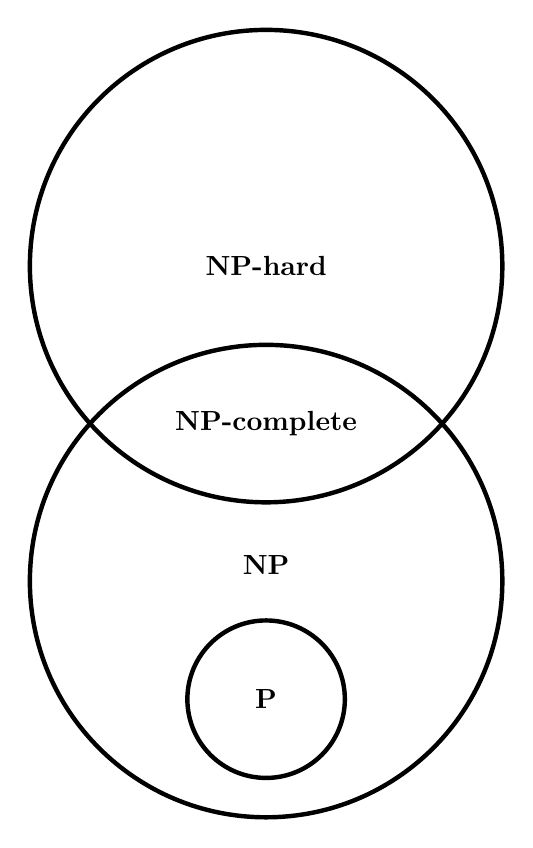
\begin{tikzpicture}
							\draw[ultra thick] (0,0) circle (3cm);
							\node at (current bounding box.center) {\textbf{NP-hard}};
							\draw[ultra thick] (0,-4) circle (3cm);
							\node at (current bounding box.center) {\textbf{NP-complete}};
							\node at ($(current bounding box.center) - (0, 1.8)$) {\textbf{NP}};
							\draw[ultra thick] (0,-5.5) circle(1cm);
							\node at ($(current bounding box.center) - (0, 3.5)$) {\textbf{P}};
						\end{tikzpicture}
					\end{adjustbox}
					\caption{\centering Visualisation of the sets P, NP, NP-hard and NP-complete.}
					\label{fig:p,np,npcomplete}
				\end{figure}
				
				Since all problems in \textit{NP} can be reduced to any \textit{NP-complete} problem, if a deterministic polynomial time algorithm can be found for an \textit{NP-complete} problem, it would also mean that the set \textit{NP} is polynomial-time solvable, proving \textit{NP} and \textit{P} are equal sets. The question of whether \textit{P} $=$ \textit{NP} has famously been immortalised as one of the millennium prize problems from the Clay Institute of Mathematics \cite{claymathMillenniumPrize}. Most researchers believe that \textit{P} $\ne$ \textit{NP} since years of effort have failed to yield efficient algorithms for \textit{NP-complete} problems \cite{cc:modern}.
			
			\subsection{Justifying Non-traditional Algorithmic Approaches}
			
%			Since even in with less randomised rules, Tetris is NP-complete, we should turn our attention to non-traditional algorithmic approaches, but first, we should show why we shouldn't be looking into traditional approaches in the first place.
%			We should mention in this section that Versus Tetris has different rules compared to the ones studied by Demaine et al. Demain et al: The difficulty of the offline version should imply the difficulty of the online version. Despite this difference, the game 
				
				It is important to note that even though \citeauthor{tetris-is-hard-even-to-approx}'s \cite{tetris-is-hard-even-to-approx} proof is based on a variant of Tetris that is quite different from Versus Tetris, the difficulty of Versus Tetris can be implied from the proof. Versus Tetris introduces additional gameplay factors, such as the competitive aspect where players can send ``garbage'' lines to their opponents, adding layers of complexity. As such, Versus Tetris is arguably more difficult than its classic variant, or  \citeauthor{tetris-is-hard-even-to-approx}'s variant \cite{tetris-is-hard-even-to-approx}.
				
				Given the NP-completeness of Tetris \cite{tetris-is-hard-even-to-approx} \cite{tetris-o1-np-hard}, it is evident that traditional deterministic algorithmic approaches would face significant challenges in efficiently playing the game \cite{cc:conceptual-perspective}. The NP-completeness of the game implies that obtaining exact solutions are computationally intractable within a reasonable time frame.
				
				To address this, we may relax the requirements for a solution. This can be done by either broadening the set of acceptable solutions or focusing on average-case scenarios instead of worst-case scenarios \cite{cc:conceptual-perspective}. This shift in focus allows the use of more practical, non-traditional algorithms that provide acceptable solutions within a reasonable time, even if they are not optimal. 
							
		\section{Approaches to Tetris}
		
			% Explain the approaches taken to tackle the Tetris problem
			% Should define each approach, and probably mention why the the algorithms were chosen.
			
			Now that the difficulty of Tetris has been established, we turn our attention to potential strategies that can be used to handle the game's complexity. In this section, we explore some of the innovative approaches that have been utilised to tackle the game of Tetris, such as imitation learning, upper confidence bound fort trees, deep reinforcement learning, and meta-heuristic algorithms.
			
			\subsection{Learning by Imitation} \label{subsec:imit-learning}
			
				In \citeyear{tetris-learning-by-imitation}, \citeauthor{tetris-learning-by-imitation} \cite{tetris-learning-by-imitation} employed a learning by imitation approach to the game of Tetris. Imitation learning aims to mimic human behaviour in some given task by learning a mapping between observations of demonstrations \cite{imitation-learning}.
				
				In their approach, played Tetris games were fed into a machine learning model as inputs, where the model would receive positive feedback when a decision matched that of the imitated system, and negative feedback otherwise \cite{tetris-learning-by-imitation}. The learning is deemed successful if the trained model maintains similarity even when faced with data outside of the training set.
				
				The learning system consists of several components, including filters, pattern calculators, and support vector machines (SVMs) (refer to Figure \ref{fig:syscomponents-learning-by-imitation}) \cite{tetris-learning-by-imitation}. Because of the time consuming nature of training SVMs, each Tetrimino had its own dedicated filters, pattern calculators and SVMs, i.e. seven SVMs \footnote{Seven SVMs for the seven Tetriminos.} are working together in the artificial player. The output of any particular SVM describes how similar a candidate move is to the choice of the imitated player.
				
				\begin{figure}
					\tikzstyle{block} = [rectangle, draw, 
					text width=6em, text centered, rounded corners, minimum height=4em]
					\tikzstyle{arrow} = [thick,->,>=stealth]
					\tikzstyle{connector} = [circle, draw, fill=red!20, minimum size=4mm, inner sep=0pt]
					\centering
					
					\begin{tikzpicture}[node distance=2cm, auto]
						
						% Nodes
						\node [block] (input) {Input: Tetris Game State};
						\node [block, below of=input] (filters) {Filters};
						\node [block, below of=filters] (pattern_calculators) {Pattern Calculators};
						\node [block, right=1cm of pattern_calculators] (features) {Hand-coded Features};
						\node [block, below of=pattern_calculators, right=.5cm of pattern_calculators.center] (svm) {Support Vector Machine};
						\node [block, below of=svm] (output) {Output: Move Decision};
						
						% Arrows
						\draw [arrow] (input) -- (filters);
						\draw [arrow] (filters) -- (pattern_calculators);
						\draw [arrow] (pattern_calculators) -- (svm);
						\draw [arrow] (features) -- (svm);
						\draw [arrow] (svm) -- (output);
					\end{tikzpicture}
					\caption{Abstraction of \citeauthor{tetris-learning-by-imitation}'s System Components}
					\label{fig:syscomponents-learning-by-imitation}
				\end{figure}
				
				Filters are made up of a multitude of patterns, which can be thought of as specific configurations in the playing field that the model uses to recognise and evaluate different game states \cite{tetris-learning-by-imitation}. Patterns do not take into account the whole matrix, but only a small area in the playing field. Thus, the authors included a list of 19 hand-coded features that takes a more global look at the game, some notable features include the number of holes that will be created after the current placement, and the number of removed lines after the current placement. Both the activated patterns and the features are passed into the support vector machine, and the move that is calculated to be the most similar is played.
				
				To evaluate their approach, \citeauthor{tetris-learning-by-imitation} used a human player as well as Fahey's artificial player \cite{fahey-ai} as systems for their model to imitate \cite{tetris-learning-by-imitation}. The outcome shows that their model can learn different styles of gameplay based on the imitated player, which is to be expected. When pitting the two learned models against each other in their variant of multiplayer Tetris \footnote{In \citeauthor{tetris-learning-by-imitation}'s variant of multiplayer Tetris, clearing $n$ lines sends $n-1$ attack rows to the opponent, with each attack row containing $n-1$ empty cells \cite{tetris-learning-by-imitation}. Attack rows are added to the bottom of the opponent's matrix.}, they found that the human imitated machine performed better than the one imitated from Fahey's AI. However, The system imitated from Fahey's AI outperformed that of the human imitated system in single player games. 
				
			\subsection{Upper Confidence Bounds for Trees}
				% TODO may need revision
				% Bandit-based Monte Carlo
				Monte-Carlo Tree Search (MCTS) is a best-first search method that is based on a randomised exploration of the search space \cite{mcts}. The algorithm evaluates states to determine the most rewarding actions, with rewards being calculated from the leaf to the root \cite{tetris-bb-mc-planning}. MCTS has the added benefit of learning from previous explorations, gradually building a game tree in memory, resulting in more accurate estimation of the most promising moves \cite{mcts}. In \citeyear{bandit-based-mcts}, \citeauthor{bandit-based-mcts} \cite{bandit-based-mcts} proposed a method, which was deemed Upper Confidence Bound for Trees (UCT), to improve the performance of the algorithm by applying a bandit algorithm known as UCB1\footnote{UCB stands for Upper Confidence Bound} to Monte-Carlo Planning. 
				
				The UCB1 formula is employed to balance the exploration-exploitation trade-offs during the search \cite{tetris-bb-mc-planning}. It helps prioritise actions that are either promising or under-explored, which effectively prunes less promising branches of the search tree. This results in a more efficient search process and a smaller, more focused tree.
				
				In \citeyear{tetris-bb-mc-planning}, \citeauthor{tetris-bb-mc-planning} \cite{tetris-bb-mc-planning} employed this approach to the game of Tetris. In their approach, the authors considered each state of the matrix, along with a given piece as a single node in the planning tree (refer to Figure \ref{fig:bbmcts-single-node}). After an action is taken, if any number of rows are cleared, a predefined reward is given to the action and the most rewarding action is selected as the resulting move. To further improve efficiency, the authors pruned the search tree further, removing actions that resulted in disadvantageous holes in the field.
				
				\begin{figure}[h]
					
					\centering
					\begin{tikzpicture}[every node/.style={inner sep=-0.4pt,anchor=south west,scale=.3},scale=.3]
						\coordinate (sw) at (5,0);
						\coordinate (nw) at (5,10);
						\coordinate (se) at (15,0);
						\coordinate (ne) at (15,10);
						\draw[fill=black!10!white] (sw) -- (nw) -- (ne) -- (se) -- cycle;
						\node at (sw){\ipiece};
						\node at ($(sw) + (4,0)$){\opiece};
						\node at ($(sw) + (2,1)$){\spiece};
						\node at ($(sw) + (1,1)$){\rotatebox{90}{\zpiece}};
						\node at ($(sw) + (0,1)$){\rotatebox{-90}{\jpiece}};
						\node at ($(sw) + (6,0)$){\tpiece};
						\node at ($(sw) + (7,1)$){\rotatebox{90}{\lpiece}};
						\node at ($(sw) + (5,1)$){\rotatebox{180}{\tpiece}};
						\node at ($(sw) + (2,3)$){\zpiece};
						\node at ($(sw) + (5,3)$){\opiece};
						\node at ($(ne) + (1,-2)$){\ipiece};
						\draw[ultra thick] (sw) -- (nw) -- (ne) -- (se) -- cycle;
					\end{tikzpicture}
					\caption{\centering An example of a single node of the matrix state and piece in the planning tree.}
					\label{fig:bbmcts-single-node}
				\end{figure}
				
				Experimental results show that the artificial player shows promise, beating Fahey's AI \cite{fahey-ai} 91 times out of 100 games using the multiplayer Tetris rules mentioned in Section \ref{subsec:imit-learning} \cite{tetris-bb-mc-planning}. The results also show that the artificial player outperformed the SVM based pattern player from \citeauthor{tetris-bb-mc-planning}'s previous work, where they approached the game with imitation learning \cite{tetris-learning-by-imitation}.
				
				% TODO may need better visualisation
			
			\subsection{Deep Reinforcement Learning}
				
				In \citeyear{tetris-drl}, \citeauthor{tetris-drl} \cite{tetris-drl} adopted a deep reinforcement approach to the game of Tetris, using a convolutional neural network to approximate a Q function, which reflects the maximum predicted discounted sum of future rewards possible by following a given policy from states to actions (refer to Equation \ref{eq:q-func}).
				\begin{equation}\label{eq:q-func}
					Q^* (s,a) = \max \mathbb{E}[r_t + \gamma r_{t+1} + \gamma^2 r_{t+2} + ... | s_t = s, a_t = a, \pi] 
				\end{equation}
				
				\noindent where $s_t$ is the state at time $t$, $a_t$ is the action taken at time $t$, $\pi$ is a policy function indicating what action to take in the current state, and is followed at every step from $t+1$ onwards, $r_t$ is the reward obtained by taking action $a_t$ at state $s_t$, and $\gamma$ is a discount factor \cite{tetris-drl}.
				
				The authors defined a state as an image of the current game screen \cite{tetris-drl}. Actions were defined in two ways, single actions, where a single input used to move a piece is considered an action, and grouped actions, where an entire sequence of actions is considered that takes a piece from its initial point at the top of the matrix to the bottom. They also used two different types of rewards, the first being the scores given from the emulator used, which was defined as the number of lines cleared. The second type of reward was defined as a heuristic function proposed by \citeauthor{lee-ai} \cite{lee-ai} (refer to Equation \ref{eq:drl-heuristic}).
				%
				\begin{equation}\label{eq:drl-heuristic}
					-0.51 \times Height + 0.76 \times Lines - 0.36 \times Holes - 0.18 \times Bumpiness
				\end{equation}
				
				This heuristic takes into account the sum of the heights of every column, the number of cleared lines, the number of holes in the matrix, and the ``bumpiness'' - sum of the absolute differences in height between adjacent columns \cite{lee-ai}. Interestingly, the weights of the heuristic were calculated by using a genetic algorithm. 
				
				The training process was further improved by using an epsilon-greedy policy, where the agent takes the best known move most of the time, but has a small probability $\epsilon$ to take a random action \cite{tetris-drl}. They also tried a novel approach where an agent that was already trained to play well could suggest moves to the algorithm. In this approach, a random action is selected with probability $\epsilon_{rand}$, an action suggested by the transferred agent is selected with probability $\epsilon_{agent}$, and the best known action to the machine is selected otherwise.
				
				Other than that, a method known as experience replay was used to create a memory for the neural network to train on. This memory consisted of every ``experience'' that the network had encountered, and was sampled when training the network. Prioritised sweeping was also utilised, where the priorities were placed on experiences which had the greatest error, and therefore the most room to improve.
				
				From the experimental results, one of the agents showed the most potential. This agent utilised a standard greedy-epsilon policy - no trained agent was used to suggest moves, grouped actions over single ones, heuristic rewards and random sampling over prioritised sweeping. It outperformed the other agents proposed in this paper, with an average score of 18. However, its capabilities were far inferior to that of \citeauthor{lee-ai}'s bot, which had an average score of 200.
				
				Later in \citeyear{tetris-drl-2}, \citeauthor{tetris-drl-2} \cite{tetris-drl-2} used a modified version of \citeauthor{tetris-drl}'s algorithm as a baseline, and proposed several different approaches taken to further optimise the algorithm. The variant of the game used to test the author's algorithms has similar rules to that of modern Tetris games, where the system will generate bags containing a piece sequence with all 7 pieces, and bags are given to the player in sequence. This piece generation system ensures that the player will not need to experience a piece drought, since a piece is guaranteed to be given in the current or next bag. The game also has a hold feature, where the player has the option to hold on to a piece for future use, and swap it out for the piece in play.
				
				\citeauthor{tetris-drl-2} proposed that the quadratic rewards from the emulator scores in \citeauthor{tetris-drl}'s paper might encourage the agent to take riskier moves, since clearing multiple lines would greatly increase the rewards given. However, this resulted in shorter survival times, as the agent waits for particular pieces. Knowing this, the author proposed utilising a linear reward function instead of a quadratic one. Comparing the results of both approaches, the authors found that the agent trained with a linear reward function outperformed that of a quadratic one, in both the survival time aspect, and the game score aspect. However, it should be noted that the quadratic models have higher points per piece dropped, meaning that they were much more efficient than the linear ones.
				
				\citeauthor{tetris-drl-2} also proposed the use of a ``harder'' Tetris game, which had a higher probability for Z and S pieces (refer to Figure \ref{fig:z-s-pieces}). The author set the probability of each piece as shown in Table \ref{tab:tet-hard-mode}. Doing this significantly decreased training time, reducing it from 3 days to a mere 6 hours.
				
				\begin{figure}
					\centering
					\begin{tikzpicture}[every node/.style={inner sep=-0.4pt,anchor=south west,scale=.5},scale=.5]
						\node at (0,0) {\zpiece};
						\node at (6,0) {\spiece};
					\end{tikzpicture}
					\caption{Z and S pieces.} \label{fig:z-s-pieces}
				\end{figure}
				
				\begin{table}
					\caption{Probability of each piece in \citeauthor{tetris-drl-2}'s ``hard'' mode.}
					\label{tab:tet-hard-mode}
					\centering
					\begin{tblr}{ c c c c c c c c }
						\hline
						& Z & S & I & J & L & O & T \\
						\hline
						Probability & 0.25 & 0.25 & 0.1 & 0.1 & 0.1 & 0.1 & 0.1\\
						\hline
					\end{tblr}
				\end{table}
				
				Finally, \citeauthor{tetris-drl-2} proposed an update rule that takes the probability of each piece into account (refer to Equation \ref{eq:q-ex-pieces}). This idea emerged from the observation that the only randomness found in a Tetris game is from piece generation. The training process involved enumerating all possible next pieces and actions to find the best action, storing the expected reward and Q-value for each state to a replay buffer and randomly sampling from the replay buffer to update the Q-network. Result of this change showed that the models trained under these update rules performed consistently better than the original models.
				%
				\begin{equation} \label{eq:q-ex-pieces}
					Q(s) \leftarrow Q(s) + \alpha [\mathbb{E}_{allPossiblePieces}[r + \gamma \max Q(s') - Q(s)]]
				\end{equation}
				
				Experimental results show that \citeauthor{tetris-drl}'s model \cite{tetris-drl} scored an average of 704.68 with modern rules in place, but \citeauthor{tetris-drl-2}'s model significantly outperformed it, with an average score of 40163.58, increasing almost 57-fold.
				
			\subsection{Meta-heuristic Algorithms} \label{subsec:metaheuristic}
				
				% MVP Algorithm and Harmony Search Algorithm
				
				According to \citeauthor{yang2020nature} \cite{yang2020nature}, the term ``meta-heuristic'' does not have any agreed upon definitions, with some scholars even using the term interchangeably with the word ``heuristic''. Even so, most definitions agree on the same things. \citeauthor{metaheuristic} \cite{metaheuristic} consolidated some of the properties that characterise most meta-heuristics as follows:
				
				\begin{enumerate}
					\item Meta-heuristics are strategies that guide the search process.
					\item The goal is to efficiently explore the search space in order to find near-optimal solutions.
					\item Meta-heuristic algorithm techniques range from simple local search procedures to complex learning processes.
					\item Meta-heuristic algorithms are non-deterministic and approximate in nature.
					\item Meta-heuristic algorithms are not designed to solve a specific problem.
				\end{enumerate}
				
				Here, we will look into two works of literature that cover the use of two distinct meta-heuristic algorithms, namely, the harmony search algorithm, and the most valuable player algorithm, in optimising Tetris agents.
				
				\subsubsection{Harmony Search Algorithm}
					
					In \citeyear{tetris-harmony-search}, \citeauthor{tetris-harmony-search} utilised the harmony search algorithm, a meta-heuristic algorithm that mimics the improvisation of music players \cite{harmony-search}, to approach Tetris \cite{tetris-harmony-search}. In the context of the algorithm, harmonies are solution vectors containing potential weights of solutions. The algorithm can be described in the following steps \cite{tetris-harmony-search}:
					
					\begin{enumerate}
						\item \textbf{Initialisation}: Program parameters are defined and the harmony memory is filled with random harmonies; each harmony is evaluated using a set objective function.
						\item \textbf{Harmony Improvisation}: A new solution is created utilising these three methods:
						\begin{enumerate}
							\item \textbf{Creation of a new solution}: A new solution is created randomly with a probability of $1 - r_{accept}$, or an existing solution in the harmony memory is selected with a probability of $1 - r_{accept}$.
							\item \textbf{Pitch adjustment}: The elements of the new harmony are modified with a probability of $r_{pa}$
							\item \textbf{Evaluation}: The new harmony is evaluated using the objective function defined.
						\end{enumerate}
						\item \textbf{Selection}: When a terminating condition is met, the best harmony in the harmony memory is selected.
					\end{enumerate}
					
					In their approach, \citeauthor{tetris-harmony-search} \cite{tetris-harmony-search} used a list of 19 feature functions, assigning numerical weights to each function. The best move for a current piece is chosen using a linear summation of these feature functions with their corresponding weights:
					
					\begin{equation}
						V(s) = \sum_{i=1}^{19}w_{i}f_{i}(s)
					\end{equation}
					
					\noindent where $s$ is the current state (board configuration), $w_i$ represents each of the weights of the $i^{th}$ feature function $f_i(s)$ and $f_i(s)$ is a function that maps a state to a real value. The objective of the optimisation process is to find an optimal set of weights that result in the most number of cleared rows. Since 19 feature functions were defined, the solutions generated by the program came in the form of a vector of 19 weights.
					
					In each iteration of the algorithm, when a set of harmonies (in the form of weights) are generated, \citeauthor{tetris-harmony-search} \cite{tetris-harmony-search} then passed the weights to their own Tetris simulator, which plays a complete game of Tetris, utilising the weights provided to decide on piece placements. After playing the game, the simulator then returns the number of rows cleared by the agent. This serves as the objective function, where more cleared rows means better agent performance. When a termination condition has been met, the program then outputs the best solution created so far.
					
					To evaluate their performance, \citeauthor{tetris-harmony-search} \cite{tetris-harmony-search} used the spawned piece to cleared rows ratio as a metric. The lower this metric was, the better the performance of the algorithm. After letting the algorithm run for two weeks straight, the program was almost able to achieve the theoretical best case, which was derived by \citeauthor{fahey-ai} \cite{fahey-ai} to be 2.5.
		
				\subsubsection{Most Valuable Player Algorithm}
				
					The most valuable player algorithm (MVPA) is a meta-heuristic algorithm inspired from sport where players form teams and compete collectively to win championship games, and individually amongst each other to win the MVP trophy \cite{mvpa}. In \citeyear{tetris-mvpa-ga}, \citeauthor{tetris-mvpa-ga} \cite{tetris-mvpa-ga} compared the use of this algorithm with the genetic algorithm (GA) in a classic Tetris environment. This algorithm can be described in the following steps:
					
					\begin{enumerate}
						\item \textbf{Initialisation}: Program parameters are defined; candidate solutions are generated.
						\item \textbf{Team Formation}: A number of teams are determined and players are divided evenly throughout the different teams.
						\item \textbf{Individual Competition}: Each player tries to develop their skills based on the existing franchise players and MVP.
						\item \textbf{Team Competition}: Two teams are selected at random to compete with one another, where the game cannot result in a loss.
						\item \textbf{Application of Greediness}: After several competitions, individual player skills are evaluated to see if any improvements were made after the games. If a player is better after the games, it will be used for the next iteration.
						\item \textbf{Application of Elitism}: 1/3 of all players with the worst skills will be replaced by 1/3 of the players with the best skills.
						\item \textbf{Remove Duplicates}: If there are individuals who are identical to one another, one of these individuals will be updated randomly.
					\end{enumerate}
					
					Similar to harmony search, a list of features are selected, and both the MVPA and GA are used to optimise the weights for each feature.
					
					Experimental results show that MVPA proved to optimise the game better than GA in terms of score and speed. In an endless game, MVPA managed to reach a score of 249 million while the GA only reached 68 million. The MVPA was also shown to find an acceptable solution faster than the GA in trials where the authors limited the spawn pieces. They observed that the MVPA converged much faster.
						
		\section{Playing Tetris with Nature-inspired Algorithms}
		
			Nature-inspired optimisation algorithms are a class of meta-heuristic algorithms. These algorithms are based on natural phenomena and biological systems, borrowing ideas like natural selection and evolution to converge on acceptable solutions \cite{nia-soft-computing}. In this section, we will highlight three such algorithms that have been adopted to attempt to tackle the game of Tetris, specifically, the aforementioned genetic algorithm (GA), ant colony optimisation (ACO), particle swarm optimisation (PSO).
			
			All these works are similar to the ones mentioned in Section \ref{subsec:metaheuristic}, in the sense that they all utilise a list of features from the board state and that they all utilise these algorithms to optimise the weights for said features to be used in a state evaluation function.
		
			% Show examples of other work that has attempted to play Tetris with NIA
			\subsection{Genetic Algorithm}
			
				In \citeyear{tetris-ga-flom-robinson}, \citeauthor{tetris-ga-flom-robinson} \cite{tetris-ga-flom-robinson} utilised a Genetic Algorithm (GA) to weight an evaluation function for Tetris. In their work, a variation of the genetic algorithm known as GENITOR was used. In a standard GA, the parents are replaced by their offspring after recombination \cite{genitor}. The GENITOR approach differs in the sense that the offspring do not replace parents, but rather replace low ranking individuals in the population.
				
				An agent's fitness was determined by the rank of the utility that the agent returned \cite{tetris-ga-flom-robinson}. \citeauthor{tetris-ga-flom-robinson} experimented with two different ways to calculate this utility. The first was to calculate the number of rows cleared by the agent before a game ends (either by losing, or by using up a finite number of pieces). The second way was to use the ratio of cleared rows per piece played. They found that both determiners had no noticeable difference in learning rate, and ultimately chose to use the first metric for the rest of their experimentation.
				
				They also experimented with different crossover operations to find out which would have the biggest positive impact on learning rate. This resulted in them using a uniform crossover approach. In their work, binary representations of the weights were used as chromosomes. Every generation, two parents were selected completely at random and recombined to make one child. With uniform crossover, a crossover mask with equally distributed 1-bits is used in the recombination process \cite{uniform-crossover}. For example,
				
				\begin{quote}
					Parent 1:\verb| 001111|\\
					Parent 2:\verb| 111100|\\
					Mask:\hspace{4pt}\verb|   010101|\\
					Child 1:\hspace{6pt}\verb| 011110|\\
					Child 2:\hspace{6pt}\verb| 101101|
				\end{quote}
				
				\noindent Child 1 is parent 1 with some bits replaced as specified by the mask and child 2 is parent 2 with some bits replaced as specified by the mask.
				
				Results show that the agents were able to continue learning each generation, and that even after 1000 runs, the agents have yet to breed into convergence  \cite{tetris-ga-flom-robinson}. \citeauthor{tetris-ga-flom-robinson} concluded that genetic algorithms work very well at searching for good weights for the evaluation function used to allow an agent to play Tetris.
				
				Later in \citeyear{tetris-ga-lewis}, \citeauthor{tetris-ga-lewis} \cite{tetris-ga-lewis} also used GA to attempt playing Tetris. In his implementation of the game, the agent was awarded a score after a line clear occurred (refer to Table \ref{tab:lewis-scores}). 
				
				\begin{table}[h]
					\caption{Score table for lines cleared in \citeauthor{tetris-ga-lewis}' Tetris game \cite{tetris-ga-lewis}.}
					\label{tab:lewis-scores}
					\centering
					\begin{tblr}{c c}
						\hline
						Lines Cleared & Score \\
						\hline
						1 & 2 \\
						2 & 5 \\
						3 & 15 \\
						4 & 60 \\
						\hline
					\end{tblr}
				\end{table}
				
				The metric used to calculate the fitness of a candidate is the score efficiency, which is defined as the average score per pieces played. that a player earns during a game of Tetris. A 4-line clear requires at least 10 Tetrominos. Thus, the theoretical maximum for this metric is 60 score $\div$ 10 pieces = 6. Experimental results show that under this metric, the algorithm mostly converged after 30 generations with a minimum scoring efficiency of 2.4, which is equivalent to 20\% of the theoretical maximum.
				
			\subsection{Ant Colony Optimisation}
				
				In \citeyear{tetris-aco}, \citeauthor{tetris-aco} \cite{tetris-aco} applied Ant Colony Optimization (ACO) to optimize the weights of a linear value function in the game of Tetris. The value function evaluates possible game states based on 16 feature functions, where each feature is scaled between 0 and 1.
				
				The weight vector, represented as $w$, is encoded into a 16-bit vector, forming a weight graph with 256 edges, where each edge corresponds to a bit value of '0' or '1'. Ants traverse this graph to find the optimal path, which corresponded to the optimal weight vector for the Tetris agent. This approach allowed the ACO algorithm to systematically explore different weight configurations and identify the most effective one for gameplay.
				
				The performance of the ACO algorithm was compared with various reinforcement learning methods. Initially, when no heuristic was applied, the ACO algorithm converged prematurely to a suboptimal solution, resulting in an average of about 7,000 lines removed. This premature convergence highlighted the limitations of ACO without additional guidance mechanisms.
				
				To address the issue of premature convergence, the researchers introduced a dynamic heuristic. This modification significantly enhanced the algorithm's performance. With the dynamic heuristic in place, the ACO algorithm's average lines removed exceeded 17,000. Moreover, the best weight configuration discovered by the algorithm achieved an impressive performance of over 23,700 lines removed. This marked improvement demonstrated the effectiveness of incorporating dynamic heuristics to guide the ants towards better solutions and avoid local optima.
				
				The results of this study were further compared to those of other traditional reinforcement learning techniques. The ACO with dynamic heuristic outperformed most of these methods, including hand-coded approaches and Genetic Algorithms (GA). The superior performance of the ACO approach, particularly with the dynamic heuristic, underscored its potential in optimizing Tetris gameplay and surpassing the effectiveness of many conventional methods.
				
			\subsection{Particle Swarm Optimisation}
			
				In \citeauthor{swarm-tetris}'s \cite{swarm-tetris} paper, the authors investigate the application of Particle Swarm Optimization (PSO) in training neural networks to play Tetris. The algorithm was used to optimize the weight values of neural networks. Unlike traditional hand-coded heuristic approaches, PSO enables the automatic discovery of effective gameplay strategies. By treating each neural network as a particle within the swarm, the algorithm iteratively improves the network's performance based on a fitness function, which in this case is the game score achieved by the Tetris-playing agent.
				
				The use of PSO for training neural networks in this context represents a significant shift from conventional methods. Traditional approaches rely heavily on hand-coded heuristics, which require extensive domain knowledge and manual tuning. PSO, on the other hand, automates the discovery process, allowing the neural networks to evolve and adapt their strategies over time. This automatic optimization is achieved through the collective behavior of the swarm, where each particle adjusts its position based on both its own experience and the experience of neighboring particles.
				
				In the experiments conducted, neural networks were trained using PSO over multiple iterations. The results indicated a continuous improvement in the performance of the agents as they learned to play Tetris more effectively. Initially, the PSO-trained agents displayed suboptimal performance compared to traditional hand-coded heuristics. However, over time and with more iterations, the agents began to exhibit increasingly sophisticated gameplay strategies. Despite these advancements, the PSO-trained agents have not yet surpassed the performance of the best hand-coded algorithms, suggesting room for further optimization and refinement in the training process.
				
				Despite these advancements, the PSO-trained agents have not yet surpassed the performance of the best hand-coded algorithms. This outcome suggests that while PSO is effective in automating the training process and uncovering new strategies, it still requires further optimization. The iterative nature of PSO allows for gradual improvement, but achieving human-level performance in Tetris remains a challenge that necessitates ongoing refinement and experimentation.
				
				The experimental results demonstrate the potential of PSO in the domain of game-playing AI, particularly in automating the training process and discovering novel strategies. The study underscores the feasibility of PSO for such applications while also pointing to the challenges that remain in achieving human-level performance in Tetris through automated training methods.
	
	\chapter{Methodology}
	
		% Graphical and textual description is provided for flow of information between components in the system/stages in the research study.
		% Graphical overview of system/research study corresponds to the textual description provided with no errors.	
		%Excellent description is provided for all methodologies, tools and techniques used to specify, design, build, test, integrate, document and deliver work products throughout the project along with the relevant supporting documents.
		% All documents provided are well-drawn/well-written, complete and correct. The purpose and role of each document in the project is stated clearly.
		
		This chapter outlines the systematic approach employed to investigate the application of nature-inspired optimization algorithms to Versus Tetris. We define the rules of the game in Section \ref{sec:rules}, show our thought process in selecting algorithms in Section \ref{sec:algo-select}, formulate the problem of Versus Tetris in Section \ref{sec:problem-formulation}, and propose methods of evaluation in Section \ref{sec:evaluation}.
		
		% Defining rules
		\section{Defining the Rules}\label{sec:rules}
		% 
			Tetris is a game that has many different variations, each with varying rules. In this section, we will formally define the game's rules that will be enforced throughout our implementation.
			
			\subsection{Tetrimino Sequence Generation}
			
				Regardless of the variant, there are seven distinct Tetriminos present in every game of Tetris, each with their own names (refer to Figure \ref{fig:tetris-pieces}). However, the way the sequences of Tetriminos are generated differ depending on the variant defined. In our variant of the game, the rules of piece generation will be similar to that defined by \citeauthor{tetris-drl-2} \cite{tetris-drl-2}.
				
				\begin{figure}
					\begin{center}
							%		
						\begin{subfigure}[t]{.1\linewidth}
							\begin{tikzpicture}[every node/.style={inner sep=-0.4pt,anchor=south west,scale=.5},scale=.5]
								\node at (0,0) {\opiece};
							\end{tikzpicture}
							\caption{O}
						\end{subfigure}
						%
						\begin{subfigure}[t]{.1\linewidth}
							\begin{tikzpicture}[every node/.style={inner sep=-0.4pt,anchor=south west,scale=.5},scale=.5]
								\node at (0,0) {\tpiece};
							\end{tikzpicture}
							\caption{T}
						\end{subfigure}
						%					
						\begin{subfigure}[t]{.1\linewidth}
							\begin{tikzpicture}[every node/.style={inner sep=-0.4pt,anchor=south west,scale=.5},scale=.5]
								\node at (0,0) {\zpiece};
							\end{tikzpicture}
							\caption{Z}
						\end{subfigure}
						%
						\begin{subfigure}[t]{.1\linewidth}
							\begin{tikzpicture}[every node/.style={inner sep=-0.4pt,anchor=south west,scale=.5},scale=.5]
								\node at (0,0) {\spiece};
							\end{tikzpicture}
							\caption{S}
						\end{subfigure}
						%					
						\begin{subfigure}[t]{.1\linewidth}
							\begin{tikzpicture}[every node/.style={inner sep=-0.4pt,anchor=south west,scale=.5},scale=.5]
								\node at (0,0) {\lpiece};
							\end{tikzpicture}
							\caption{L}
						\end{subfigure}
						%					
						\begin{subfigure}[t]{.1\linewidth}
							\begin{tikzpicture}[every node/.style={inner sep=-0.4pt,anchor=south west,scale=.5},scale=.5]
								\node at (0,0) {\jpiece};
							\end{tikzpicture}
							\caption{J}
						\end{subfigure}
						%	
						\begin{subfigure}[t]{.1\linewidth}
							\begin{tikzpicture}[every node/.style={inner sep=-0.4pt,anchor=south west,scale=.5},scale=.5]
								\node at (0,0) {\ipiece};
							\end{tikzpicture}
							\caption{I}
						\end{subfigure}		
					\end{center}
					\caption{The Tetriminos and their names.}
					\label{fig:tetris-pieces}
				\end{figure}
				
				The system used to generate piece sequences is known as \textit{7-bag}. It works by generating a sequence of all seven Tetriminos permuted randomly, as if they were drawn from a bag \cite{harddrop}. The sequence is then given to the player before another bag is generated. This means that there are $7!$ or 5,040 different permutations of the seven pieces for any given bag. The system gives each one of these permutations an equal probability of occurring. This ensures that there will not be periods of piece drought -- where a player waits for an extended period of time for a preferred piece,\footnote{The maximum number of pieces between a piece $X$ and another piece $X$ is 12.} or piece rain -- where a player keeps receiving the same pieces consecutively.
			
			\subsection{Matrix Dimensions}
			
				Under official guideline Tetris rules, the matrix dimension is 10 columns wide and 22 rows tall, but the top two rows are hidden. These two rows will allow the player to survive even if the middle of the matrix is filled up by moving the piece to the side of the matrix (refer to Figure \ref{fig:22-row-ex}).
				
				\begin{figure}
					\centering
					
\begin{tikzpicture}[every node/.style={inner sep=-0.4pt,anchor=south west,scale=.3},scale=.3]
						\coordinate (sw) at (5,0);
						\coordinate (nw) at (5,20);
						\coordinate (se) at (15,0);
						\coordinate (ne) at (15,20);
						\draw[fill=black!10!white] (sw) -- (nw) -- (ne) -- (se) -- cycle;
						\node at (sw){\garbage{20}{8}};
						\node at ($(nw) + (3,0)$) {\ipiece};
						\draw[ultra thick] (sw) -- (nw) -- (ne) -- (se) -- cycle;
					\end{tikzpicture}
					\caption{\centering I piece is spawned at the 21st row of the matrix, but the player can survive by slotting the piece into the eighth column of the matrix.}
					\label{fig:22-row-ex}
				\end{figure}			
			
			\subsection{Spins}
			
				The rotation system used by guideline Tetris games is known as the \textit{Super Rotation System} (SRS), and it defines how Tetriminos spawn, rotate, and what kicks can be performed \cite{harddrop}. It is important for us to define the rotation rules here so that we can create a simulation of Tetris that is as accurate as possible.
				
				When unobstructed, the Tetriminos all rotate around a single point (refer to Figure \ref{fig:srs}). The O and I pieces rotate around an intersection of grid-lines whereas the other pieces rotate around the centre of a grid-box.
								
				However, if the piece is obstructed by the wall, the floor, or another fixed piece, the game attempts to ``kick'' the Tetrimino into an alternative position nearby \cite{harddrop}. When this occurs, the game tests 5 potential positions to kick the piece towards; if the position of all the tests are unavailable, the rotation itself fails, resulting in the piece not rotating at all. Other than the O piece, all the other pieces are able to kick into different positions. The I piece has its own set of kick values, but the remaining pieces all share identical ones.
				
				Tables \ref{tab:i-kick} and \ref{tab:non-i-kick} show the kick values for these pieces \cite{harddrop}. The kick values represent translations relative to rotations. The following conventions will be used for naming rotation states for the tables:
				
				\begin{itemize}
					\item 0 = spawn state
					\item L = state resulting from a counter-clockwise rotation from the spawn state
					\item R = state resulting from a clockwise rotation from the spawn state.
					\item 2 = state resulting from 2 successive rotations in either direction from spawn.
				\end{itemize}
				
				\begin{table}
					\caption{I Tetrimino Wall Kick Data.}
					\label{tab:i-kick}
					\centering
					\begin{tblr}{colspec={| c | c | c | c | c | c |},cell{2-Z}{2-Z}={font=\ttfamily},row{1}={gray!35}}
						\hline
						& Test 1 & Test 2 & Test 3 & Test 4 & Test 5 \\
						\hline
						0 $\rightarrow$ R & (0, 0) & (-2, 0) & \texttt{(+1, 0)} & (-2, -1) & (+1, +2) \\
						\hline
						R $\rightarrow$ 0 & (0, 0) & (+2, 0) & (-1, 0) & (+2, +1) & (-1, -2) \\
						\hline
						R $\rightarrow$ 2 & (0, 0) & (-1, 0) & (+2, 0) & (-1, +2) & (+2, -1) \\
						\hline
						2 $\rightarrow$ R & (0, 0) & (+1, 0) & (-2, 0) & (+1, -2) & (-2, +1) \\
						\hline
						2 $\rightarrow$ L & (0, 0) & (+2, 0) & (-1, 0) & (+2, +1) & (-1, -2) \\
						\hline
						L $\rightarrow$ 2 & (0, 0) & (-2, 0) & (+1, 0) & (-2, -1) & (+1, +2) \\
						\hline
						L $\rightarrow$ 0 & (0, 0) & (+1, 0) & (-2, 0) & (+1, -2) & (-2, +1) \\
						\hline
						0 $\rightarrow$ L & (0, 0) & (-1, 0) & (+2, 0) & (-1, +2) & (+2, -1) \\
						\hline
					\end{tblr}
				\end{table}
				
				\begin{table}
					\caption{T, Z, S, L and J Tetrimino Wall Kick Data.}
					\label{tab:non-i-kick}
					\centering
					\begin{tblr}{colspec={| c | c | c | c | c | c |},cell{2-Z}{2-Z}={font=\ttfamily},row{1}={gray!35}}
						\hline
						& Test 1 & Test 2 & Test 3 & Test 4 & Test 5 \\
						\hline
						0 $\rightarrow$ R & (0, 0) & (-1, 0) & (-1, +1) & (0, -2) & (-1, -2) \\
						\hline
						R $\rightarrow$ 0 & (0, 0) & (+1, 0) & (+1, -1) & (0, +2) & (+1, +2) \\
						\hline
						R $\rightarrow$ 2 & (0, 0) & (+1, 0) & (+1, -1) & (0, +2) & (+1, +2) \\
						\hline
						2 $\rightarrow$ R & (0, 0) & (-1, 0) & (-1, +1) & (0, -2) & (-1, -2) \\
						\hline
						2 $\rightarrow$ L & (0, 0) & (+1, 0) & (+1, +1) & (0, -2) & (+1, -2) \\
						\hline
						L $\rightarrow$ 2 & (0, 0) & (-1, 0) & (-1, -1) & (0, +2) & (-1, +2) \\
						\hline
						L $\rightarrow$ 0 & (0, 0) & (-1, 0) & (-1, -1) & (0, +2) & (-1, +2) \\
						\hline
						0 $\rightarrow$ L & (0, 0) & (+1, 0) & (+1, +1)	& (0, -2) & (+1, -2) \\
						\hline
					\end{tblr}
				\end{table}
				
				\begin{figure}
					\centering
					\begin{tikzpicture}[every node/.style={inner sep=-0.4pt,anchor=south west,scale=.4},scale=.4]
						% opiece
						\node at (0,0) {\opiece};
						\filldraw[black] (1,1) circle (4pt);
						\node at (5,0) {\opiece};
						\filldraw[black] (6,1) circle (4pt);
						\node at (10,0) {\opiece};
						\filldraw[black] (11,1) circle (4pt);
						\node at (15,0) {\opiece};
						\filldraw[black] (16,1) circle (4pt);
						% tpiece
						\node at (0,-3) {\tpiece};
						\filldraw[black] (1.5,-2.5) circle (4pt);
						\node at (5,-4) {\rotatebox{-90}{\tpiece}};
						\filldraw[black] (5.5,-2.5) circle (4pt);
						\node at (9,-4) {\rotatebox{180}{\tpiece}};
						\filldraw[black] (10.5,-2.5) circle (4pt);
						\node at (14,-4) {\rotatebox{90}{\tpiece}};
						\filldraw[black] (15.5,-2.5) circle (4pt);
						% zpiece
						\node at (0, -7) {\zpiece};
						\filldraw[black] (1.5,-6.5) circle (4pt);
						\node at (5, -8) {\rotatebox{90}{\zpiece}};
						\filldraw[black] (5.5,-6.5) circle (4pt);
						\node at (9, -8) {\zpiece};
						\filldraw[black] (10.5,-6.5) circle (4pt);
						\node at (14, -8) {\rotatebox{90}{\zpiece}};
						\filldraw[black] (15.5,-6.5) circle (4pt);
						% spiece
						\node at (0,-11){\spiece};
						\filldraw[black] (1.5,-10.5) circle (4pt);
						\node at (5,-12){\rotatebox{90}{\spiece}};
						\filldraw[black] (5.5,-10.5) circle (4pt);
						\node at (9,-12){\spiece};
						\filldraw[black] (10.5,-10.5) circle (4pt);
						\node at (14,-12){\rotatebox{90}{\spiece}};
						\filldraw[black] (15.5,-10.5) circle (4pt);
						% lpiece
						\node at (0,-15){\lpiece};
						\filldraw[black] (1.5,-14.5) circle (4pt);
						\node at (5,-16){\rotatebox{-90}{\lpiece}};
						\filldraw[black] (5.5,-14.5) circle (4pt);
						\node at (9,-16){\rotatebox{180}{\lpiece}};
						\filldraw[black] (10.5,-14.5) circle (4pt);
						\node at (14,-16){\rotatebox{90}{\lpiece}};
						\filldraw[black] (15.5,-14.5) circle (4pt);
						% jpiece
						\node at (0,-19){\jpiece};
						\filldraw[black] (1.5,-18.5) circle (4pt);
						\node at (5,-20){\rotatebox{-90}{\jpiece}};
						\filldraw[black] (5.5,-18.5) circle (4pt);
						\node at (9,-20){\rotatebox{180}{\jpiece}};
						\filldraw[black] (10.5,-18.5) circle (4pt);
						\node at (14,-20){\rotatebox{90}{\jpiece}};
						\filldraw[black] (15.5,-18.5) circle (4pt);
						% ipiece
						\node at (0,-23) {\ipiece};
						\filldraw[black] (2,-23) circle (4pt);
						\node at (6,-25) {\rotatebox{90}{\ipiece}};
						\filldraw[black] (6,-23) circle (4pt);
						\node at (9,-24) {\rotatebox{180}{\ipiece}};
						\filldraw[black] (11,-23) circle (4pt);
						\node at (15,-25) {\rotatebox{-90}{\ipiece}};
						\filldraw[black] (16,-23) circle (4pt);
					\end{tikzpicture}
					\caption{\centering The four rotation states of all seven Tetriminos. The black dots represent centres of rotation.}
					\label{fig:srs}
				\end{figure}
			
			\subsection{Attacks}
			
				In \citeauthor{tetris-learning-by-imitation}'s papers \cite{tetris-learning-by-imitation} \cite{tetris-bb-mc-planning}, they defined attack rules for their variant of multiplayer Tetris. Here, we will define the attack rules of guideline Tetris, which will be used for our implementation.
				
				\subsubsection{Garbage}
					
					Garbage lines (or attack lines) are lines sent from one opponent to another. They all have a one column well that would allow a player to clear them (refer to Figure \ref{fig:gar}). Garbage is sent in batches, when a player performs an action that is able to send garbage lines, those garbage lines are grouped together, and the wells of grouped garbage lines are always on the same column. However, if the same player performs more attack actions, there may be multiple different wells present in garbage lines. Garbage lines are a key part of the game as players can also use these lines to send attacks back to the opponent.
					
					\begin{figure}
						\centering
						\begin{minipage}{.2\textwidth}
							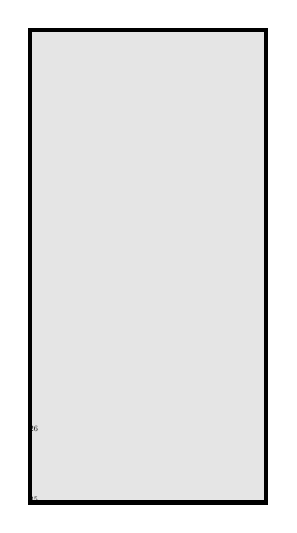
\begin{tikzpicture}[every node/.style={inner sep=-0.4pt,anchor=south west,scale=.3},scale=.3]
								\coordinate (sw) at (5,0);
								\coordinate (nw) at (5,20);
								\coordinate (se) at (15,0);
								\coordinate (ne) at (15,20);
								\coordinate (gar) at (5,5);
								\draw[fill=black!10!white] (sw) -- (nw) -- (ne) -- (se) -- cycle;
								\node at (sw){\garbage{3}{5}};
								\node at ($(sw) + (0,3)$){\garbage{2}{6}};
								\node at ($(gar) + (4,-2)$){\rotatebox{90}{\lpiece}};
								\draw[ultra thick] (sw) -- (nw) -- (ne) -- (se) -- cycle;
							\end{tikzpicture}
						\end{minipage}\hspace{20pt}$\rightarrow$\hspace{20pt}
						\begin{minipage}{.2\textwidth}
							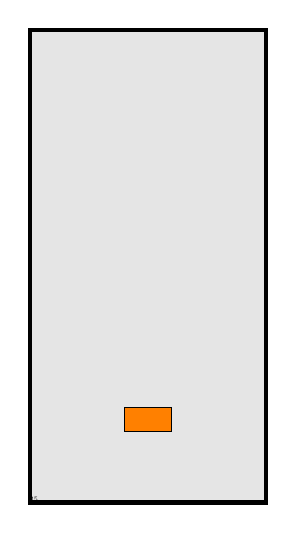
\begin{tikzpicture}[every node/.style={inner sep=-0.4pt,anchor=south west,scale=.3},scale=.3]
								\coordinate (sw) at (5,0);
								\coordinate (nw) at (5,20);
								\coordinate (se) at (15,0);
								\coordinate (ne) at (15,20);
								\coordinate (gar) at (5,3);;
								\draw[fill=black!10!white] (sw) -- (nw) -- (ne) -- (se) -- cycle;
								\node at (sw){\garbage{3}{5}};
								\draw[fill = orange] (9,3) rectangle (11,4);
								\draw[ultra thick] (sw) -- (nw) -- (ne) -- (se) -- cycle;
							\end{tikzpicture}
						\end{minipage}
						\caption{Example of garbage lines (gray) being cleared by an L piece.}
						\label{fig:gar}
					\end{figure}
			
				\subsubsection{Line Clears}
				
					Any action that clears two or more lines simultaneously will send garbage lines to the opponent (refer to Table \ref{tab:line-clear}). It may seem obvious that it is always better for the player to go for Tetrises (4-line clears), but we will shed light on another mechanic that will impact strategy largely in Section \ref{subsubsec:combos}. 
					
					\begin{table}
						\centering
						\caption{Attack Table for Line Clears}
						\label{tab:line-clear}
						\begin{tblr}{c c}
							\hline
							Lines Cleared & Garbage Sent\\
							\hline
							1 & 0\\
							2 & 1\\
							3 & 2\\
							4 & 4
						\end{tblr}
					\end{table}
				
				\subsubsection{T-spins}
				
					T-spins are a feature implemented in modern Tetris games that allow players to increase their scoring without simply performing Tetrises. To define a T-spin, we can first imagine the T piece in a 3 $\times$ 3 box (refer to Figure \ref{fig:t}).
					
					\begin{figure}[h]
						\centering
						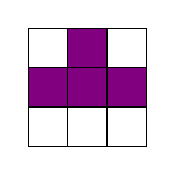
\begin{tikzpicture}[every node/.style={inner sep=-0.4pt,anchor=south west,scale=.5},scale=.5]
							\draw (0,0) rectangle (1,1);
							\draw (1,0) rectangle (2,1);
							\draw (2,0) rectangle (3,1);
							\draw[fill = violet] (0,1) rectangle (1,2);
							\draw[fill = violet] (1,1) rectangle (2,2);
							\draw[fill = violet] (2,1) rectangle (3,2);
							\draw (0,2) rectangle (1,3);
							\draw[fill = violet] (1,2) rectangle (2,3);
							\draw (2,2) rectangle (3,3);						
						\end{tikzpicture}
						\caption{T-piece in a 3 $\times$ 3 box.}
						\label{fig:t}
					\end{figure}
					
					For a T-spin to occur, the last movement of a T piece must have been a rotation, and at least three of the four corners in the 3 $\times$ 3 box needs to be filled (refer to Figure \ref{fig:t-spin}).
					
					\begin{figure}[h]
						\centering
						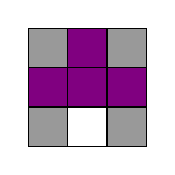
\begin{tikzpicture}[every node/.style={inner sep=-0.4pt,anchor=south west,scale=.5},scale=.5]
							\draw[fill = black!40!white] (0,0) rectangle (1,1);
							\draw (1,0) rectangle (2,1);
							\draw[fill = black!40!white] (2,0) rectangle (3,1);
							\draw[fill = violet] (0,1) rectangle (1,2);
							\draw[fill = violet] (1,1) rectangle (2,2);
							\draw[fill = violet] (2,1) rectangle (3,2);
							\draw[fill = black!40!white] (0,2) rectangle (1,3);
							\draw[fill = violet] (1,2) rectangle (2,3);
							\draw[fill = black!40!white] (2,2) rectangle (3,3);						
						\end{tikzpicture}
						\caption{\centering Visualisation of the T-spin condition. At least three of the four grey squares need to be filled.}
						\label{fig:t-spin}
					\end{figure}
				
					Regular T-spins send double the lines that they clear (refer to Table \ref{tab:t-spin}). Figure \ref{fig:t-spin} shows a few examples of T-spins.
					
					\begin{figure}
						\centering
						\begin{subfigure}{\textwidth}
							\centering
							\begin{minipage}{.2\textwidth}
								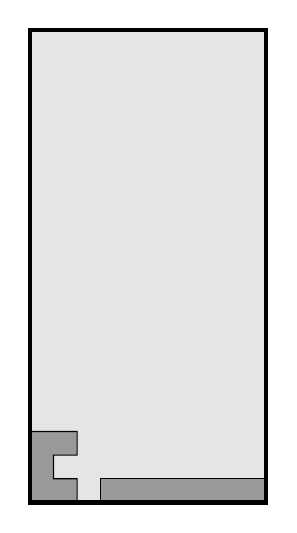
\begin{tikzpicture}[every node/.style={inner sep=-0.4pt,anchor=south west,scale=.3},scale=.3]
									\coordinate (sw) at (5,0);
									\coordinate (nw) at (5,20);
									\coordinate (se) at (15,0);
									\coordinate (ne) at (15,20);
									\draw[fill=black!10!white] (sw) -- (nw) -- (ne) -- (se) -- cycle;
									\draw[fill=black!40!white] (sw) -- (5,3) -- (6,3) -- (7,3) -- (7,2) -- (6,2) -- (6,1) -- (7,1) -- (7,0) -- cycle;
									\draw[fill=black!40!white] (se) rectangle (8,1);
									\node at (7,0){\rotatebox{-90}{\tpiece}};
									\draw[ultra thick] (sw) -- (nw) -- (ne) -- (se) -- cycle;
								\end{tikzpicture}
							\end{minipage}\hspace{20pt} \texttt{right rotate} $\rightarrow$ \hspace{20pt}
							\begin{minipage}{.2\textwidth}
								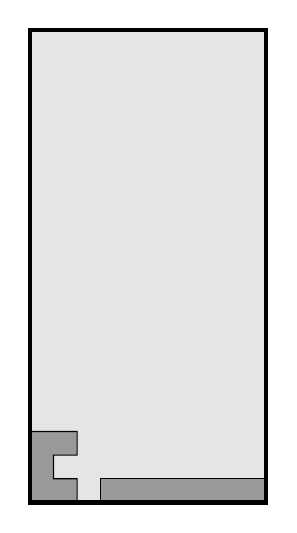
\begin{tikzpicture}[every node/.style={inner sep=-0.4pt,anchor=south west,scale=.3},scale=.3]
									\coordinate (sw) at (5,0);
									\coordinate (nw) at (5,20);
									\coordinate (se) at (15,0);
									\coordinate (ne) at (15,20);
									\draw[fill=black!10!white] (sw) -- (nw) -- (ne) -- (se) -- cycle;
									\draw[fill=black!40!white] (sw) -- (5,3) -- (6,3) -- (7,3) -- (7,2) -- (6,2) -- (6,1) -- (7,1) -- (7,0) -- cycle;
									\draw[fill=black!40!white] (se) rectangle (8,1);
									\node at (6,0){\rotatebox{180}{\tpiece}};
									\draw[ultra thick] (sw) -- (nw) -- (ne) -- (se) -- cycle;
								\end{tikzpicture}
							\end{minipage}
							\caption{Example of a T-spin Single.}
						\end{subfigure}
						\begin{subfigure}{\textwidth}
							\centering
							\begin{minipage}{.2\textwidth}
								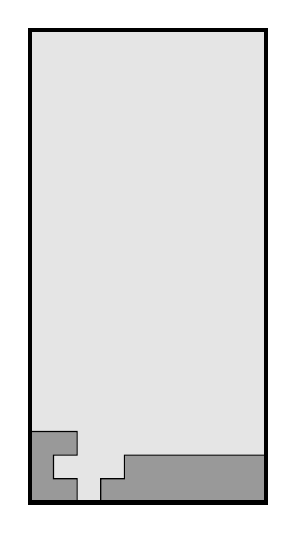
\begin{tikzpicture}[every node/.style={inner sep=-0.4pt,anchor=south west,scale=.3},scale=.3]
									\coordinate (sw) at (5,0);
									\coordinate (nw) at (5,20);
									\coordinate (se) at (15,0);
									\coordinate (ne) at (15,20);
									\draw[fill=black!10!white] (sw) -- (nw) -- (ne) -- (se) -- cycle;
									\draw[fill=black!40!white] (sw) -- (5,3) -- (6,3) -- (7,3) -- (7,2) -- (6,2) -- (6,1) -- (7,1) -- (7,0) -- cycle;
									\draw[fill=black!40!white] (se) -- (15,2) -- (9,2) -- (9,1) -- (8,1) -- (8,0) -- cycle;
									\node at (7,0){\rotatebox{-90}{\tpiece}};
									\draw[ultra thick] (sw) -- (nw) -- (ne) -- (se) -- cycle;
								\end{tikzpicture}
							\end{minipage}\hspace{20pt} \texttt{right rotate} $\rightarrow$ \hspace{20pt}
							\begin{minipage}{.2\textwidth}
								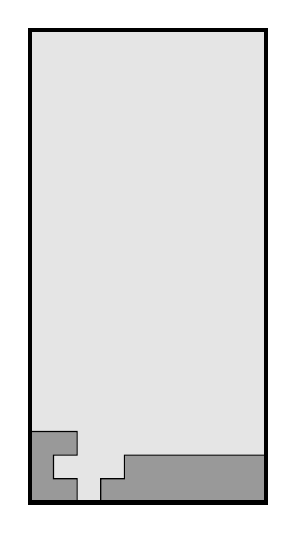
\begin{tikzpicture}[every node/.style={inner sep=-0.4pt,anchor=south west,scale=.3},scale=.3]
									\coordinate (sw) at (5,0);
									\coordinate (nw) at (5,20);
									\coordinate (se) at (15,0);
									\coordinate (ne) at (15,20);
									\draw[fill=black!10!white] (sw) -- (nw) -- (ne) -- (se) -- cycle;
									\draw[fill=black!40!white] (sw) -- (5,3) -- (6,3) -- (7,3) -- (7,2) -- (6,2) -- (6,1) -- (7,1) -- (7,0) -- cycle;
									\draw[fill=black!40!white] (se) -- (15,2) -- (9,2) -- (9,1) -- (8,1) -- (8,0) -- cycle;
									\node at (6,0){\rotatebox{180}{\tpiece}};
									\draw[ultra thick] (sw) -- (nw) -- (ne) -- (se) -- cycle;
								\end{tikzpicture}
							\end{minipage}
							\caption{Example of a T-spin Double.}
						\end{subfigure}
						\begin{subfigure}{\textwidth}
							\centering
							\begin{minipage}{.2\textwidth}
								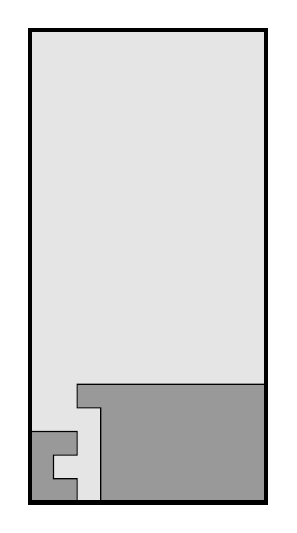
\begin{tikzpicture}[every node/.style={inner sep=-0.4pt,anchor=south west,scale=.3},scale=.3]
									\coordinate (sw) at (5,0);
									\coordinate (nw) at (5,20);
									\coordinate (se) at (15,0);
									\coordinate (ne) at (15,20);
									\draw[fill=black!10!white] (sw) -- (nw) -- (ne) -- (se) -- cycle;
									\draw[fill=black!40!white] (sw) -- (7,0) -- (7,1) -- (6,1) -- (6,2) -- (7,2) -- (7,3) -- (5,3) -- cycle;
									\draw[fill=black!40!white] (se) -- (15,5) -- (7,5) -- (7,4) -- (8,4) -- (8,3) -- (8,0) -- cycle;
									\node at ($(sw) + (0,3)$){\tpiece};
									\draw[ultra thick] (sw) -- (nw) -- (ne) -- (se) -- cycle;
								\end{tikzpicture}
							\end{minipage}\hspace{20pt} \texttt{left rotate} $\rightarrow$ \hspace{20pt}
							\begin{minipage}{.2\textwidth}
								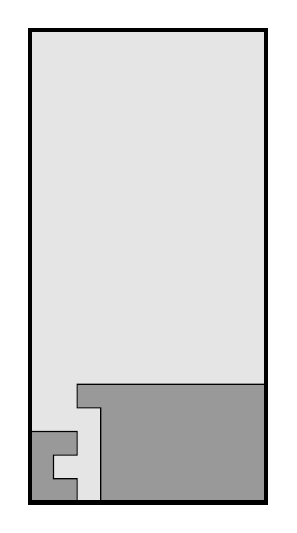
\begin{tikzpicture}[every node/.style={inner sep=-0.4pt,anchor=south west,scale=.3},scale=.3]
									\coordinate (sw) at (5,0);
									\coordinate (nw) at (5,20);
									\coordinate (se) at (15,0);
									\coordinate (ne) at (15,20);
									\draw[fill=black!10!white] (sw) -- (nw) -- (ne) -- (se) -- cycle;
									\draw[fill=black!40!white] (sw) -- (7,0) -- (7,1) -- (6,1) -- (6,2) -- (7,2) -- (7,3) -- (5,3) -- cycle;
									\draw[fill=black!40!white] (se) -- (15,5) -- (7,5) -- (7,4) -- (8,4) -- (8,3) -- (8,0) -- cycle;
									\node at (6,0){\rotatebox{90}{\tpiece}};
									\draw[ultra thick] (sw) -- (nw) -- (ne) -- (se) -- cycle;
								\end{tikzpicture}
							\end{minipage}
							\caption{Example of a T-spin Triple.}
							\label{fig:t-spin-triple}
						\end{subfigure}
						\caption{Examples of T-spins.}
					\end{figure}
					
					\begin{table}
						\centering
						\caption{Attack Table for T-spins}
						\label{tab:t-spin}
						\begin{tblr}{c c}
							\hline
							T-Spin & Garbage Sent\\
							\hline
							Single & 2\\
							Double & 4\\
							Triple & 6\\
						\end{tblr}
					\end{table}
					
				\subsubsection{Back-to-back (B2B)}
				
					Back-to-back is a feature that encourages players to continuously play for Tetrises and T-spins. When these attacks are done back-to-back, it increases the garbage lines being sent to the opponent by one. For example, if a player performs a Tetris, and their following attack is also a Tetris, they would send a total of 9 lines; 4 from the initial attack, and 4 + 1 back-to-back from the latter.
				
				\subsubsection{Combos}\label{subsubsec:combos}
				
					When a player clears multiple lines in quick succession, with every subsequent piece being used to clear at least one line, they initiate a combo. At certain points in a combo, additional lines are added to the garbage group sent to the opponent (refer to Table \ref{tab:combo}). 
					
					\begin{table}[h]
						\centering
						\begin{tblr}{| c | c |}
							\hline
							Combo & Additional Garbage\\
							\hline
							0 & 0\\
							1 & 0\\
							2 & 1\\
							3 & 1\\
							4 & 2\\
							5 & 2\\
							6 & 3\\
							7 & 3\\
							8 & 4\\
							9 & 4\\
							10 & 4\\
							11+ & 5\\
							\hline
						\end{tblr}
						\caption{Combo Table}
						\label{tab:combo}
					\end{table}
				
				\subsubsection{Perfect Clears}
				
					A perfect clear occurs when a player clears the matrix completely, leaving no remnants of existing Tetrominos behind. It can be difficult to perform perfect clears in Versus Tetris, because if there is an odd number of garbage sent from the opponent, a perfect clear becomes completely impossible. Because of this, a perfect clear has the highest attack in a single move, sending 10 lines of garbage to the opponent.
				
				\subsubsection{Stored attack}
				
					When garbage is being sent to an opponent, the garbage lines do not suddenly appear in the opponent's matrix. It is stored in an attack potential, usually represented as a vertical meter on the side of the matrix (refer to Figure \ref{fig:attack-potential}). This is to let the opponent see the potential attacks that might be coming, and allows them to clear lines in order to perform cancelling.
					
					Cancelling is done when the garbage sent in a move is equivalent or higher to the number of garbage lines stored in the attack potential. This allows players to defend their matrix from unfavourable garbage. Figure \ref{fig:attack-potential} shows an example of cancelling a 6-line attack potential with a T-spin Triple (refer to Figure \ref{fig:t-spin-triple}).
					
					\begin{figure}
						\centering
						\begin{minipage}{.2\textwidth}
							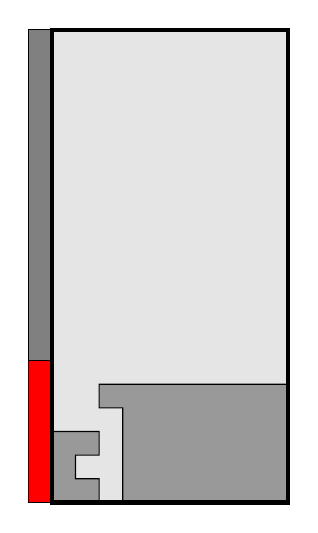
\begin{tikzpicture}[every node/.style={inner sep=-0.4pt,anchor=south west,scale=.3},scale=.3]
								\coordinate (sw) at (5,0);
								\coordinate (nw) at (5,20);
								\coordinate (se) at (15,0);
								\coordinate (ne) at (15,20);
								\draw[fill=black!10!white] (sw) -- (nw) -- (ne) -- (se) -- cycle;
								\draw[fill=black!40!white] (sw) -- (7,0) -- (7,1) -- (6,1) -- (6,2) -- (7,2) -- (7,3) -- (5,3) -- cycle;
								\draw[fill=black!40!white] (se) -- (15,5) -- (7,5) -- (7,4) -- (8,4) -- (8,3) -- (8,0) -- cycle;
								\node at (6,0){\rotatebox{90}{\tpiece}};
								\draw[fill=gray] (sw) rectangle (4,20);
								\draw[fill=red] (sw) rectangle (4,6);
								\draw[ultra thick] (sw) -- (nw) -- (ne) -- (se) -- cycle;
							\end{tikzpicture}
						\end{minipage}
						\hspace{20pt} $\rightarrow$ \hspace{20pt}
						\begin{minipage}{.2\textwidth}
							\begin{minipage}{.2\textwidth}
								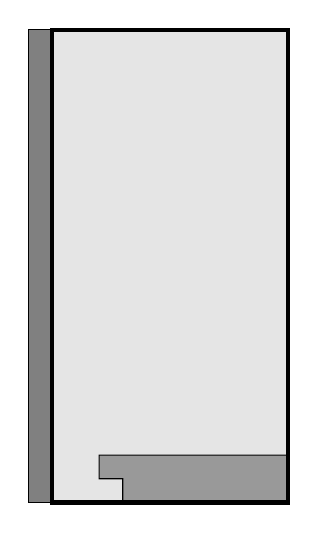
\begin{tikzpicture}[every node/.style={inner sep=-0.4pt,anchor=south west,scale=.3},scale=.3]
									\coordinate (sw) at (5,0);
									\coordinate (nw) at (5,20);
									\coordinate (se) at (15,0);
									\coordinate (ne) at (15,20);
									\draw[fill=black!10!white] (sw) -- (nw) -- (ne) -- (se) -- cycle;
									\draw[fill=black!40!white] (se) -- (15,2) -- (7,2) -- (7,1) -- (8,1) -- (8,0) -- cycle;
									\draw[fill=gray] (sw) rectangle (4,20);
									\draw[ultra thick] (sw) -- (nw) -- (ne) -- (se) -- cycle;
								\end{tikzpicture}
							\end{minipage}
						\end{minipage}
						\caption{\centering Example of Stored Attack and Cancelling.}
						\label{fig:attack-potential}
					\end{figure}
			
			\subsection{Gravity}
			
				In modern Versus Tetris games, gravity starts slow but slowly increases in order to force the players to make decisions quicker. However, in our implementation, we are more interested in the quality of the decisions being made, not the speed at which it is being made. Therefore, in this implementation, gravity will not be a factor. There are two ways that this might be implemented:
				
				\begin{enumerate}
					\item \textbf{Zero Gravity}: The player has to manually move pieces down with a key, and manually place a piece with another key.
					\item \textbf{Legal Placement Selection}: Instead of requiring the players to manually move pieces, we give the player several options for a piece to be placed, and check for legality before giving the options to the player.
				\end{enumerate}
				
				When the game is outputted, the speed of the algorithms will follow the pace of the opposing player, similar to a turn-based game like chess. The player will play a move, and the algorithm will play a move. With no gravity, the player will be able to take as long as they want to plan ahead.
			
			\subsection{Other Features}
			
				Here two additional features that may help a player improve decision making will be listed.
				
				\begin{itemize}
					\item \textbf{Hold}: Much like in \citeauthor{tetris-drl-2}'s \cite{tetris-drl-2} work, the hold function is used to hold on to a piece for future use and may be swapped any time with a piece in play.
					\item \textbf{Five-piece Lookahead}:In our implementation of the game, five pieces of lookahead will be given to the player at all times, i.e. the player will be able to see five-pieces in their queue. This does two things:
					\begin{enumerate}
						\item It allows our player to plan for future pieces.
						\item It allows our player to calculate the probability of upcoming pieces.
					\end{enumerate}
				\end{itemize}
%				hold
%				5-piece lookahead
		
		\section{Algorithm Selection}\label{sec:algo-select}
		% how algorithms work, why we choose them
			Choosing the right algorithms is crucial for tackling the challenges of Versus Tetris. In this study, the three aforementioned nature-inspired optimization algorithms have been selected -- Genetic Algorithms (GA), Particle Swarm Optimization (PSO), and Ant Colony Optimization (ACO). These algorithms were chosen because previous research has shown they hold promise in playing Tetris.
			
			These algorithms have been well-studied and validated in other domains, giving us confidence in their potential for this study. Their selection also reflects our goal of exploring a diverse set of optimization approaches, which can yield deeper insights into their performance and suitability for real-time gaming environments. The algorithms will all have the same information as one another, and will all be evaluated with the same piece sequences.
		
		\section{Problem Formulation}\label{sec:problem-formulation}
		
			In this section, we will formulate the problem of Versus Tetris. Even though multiple different algorithms will be used in order to optimise the decision making process of the game, the parameter tuning for each algorithm addressed in the results section.
		
			\subsection{Problem Definition}
			
				The problem is to develop a Tetris agent capable of playing Tetris well by effectively evaluating state-action pairs using a weighted feature function and optimising the agent's strategy based on win/loss outcomes.
				
			\subsection{States and Actions}
			
				In our problem, a state is a comprehensive representation of the Tetris matrix, including:
				
				\begin{enumerate}
					\item \textbf{Matrix configurations}: Information on both matrices, including occupied and unoccupied ci neells.
					\item \textbf{Current Tetrominos}: The current Tetrominos each agent is using
					\item \textbf{Lookahead}: The current five lookahead pieces in the queue of each player.
					\item \textbf{Hold}: The current piece being held by each player.
				\end{enumerate}
				
				To an agent, an action is simply seen as a legal piece placement. An agent does not need to know how to move a piece from one place to another, they just need to know whether it is possible to get there. Of course, holding the current piece is also a legal action.
				
				In order to decide on an action, the agent will be utilising a heuristic which is a weighted sum of numerical features, much like in previous studies (refer to Equation \ref{eq:heuristic}).
				
				\begin{equation} 
					\sum_{i=1}^{k} w_i f(S)_i
				\end{equation}\label{eq:heuristic}
				
				\noindent where $S$ is a state, $f_i$ is the feature function of said state, and $w_i$ is the corresponding weight of feature $f_i$. The weights for each feature will be optimised using nature-inspired algorithms.
				
				When an action is decided on and taken, the state transitions from one state to the next. The transitional model would place the piece, check for line clears, and update attack potentials as needed.
				
				\begin{equation}
					S_{t+1} = T(S_t, A)
				\end{equation}
				
				When either the agent or an opponent has lost, a termination condition is met.
				
			\subsection{Features}
				
				Plenty of the literature that utilise any form of meta-heuristics have identified a number of features that describe informative aspects of a Tetris grid that can all be numerically defined. We believe that Versus Tetris is different enough that it will need a different set of features that should be taken into consideration, although there will be some overlapping features. These features include:
				
				\begin{enumerate}
					\item \textbf{Pile height}: The row number of the highest occupied cell in the grid.
					\item \textbf{Hole count}: A hole is an unoccupied cell with an occupied cell on top of it.
					\item \textbf{Column transitions}: The sum of all vertical transitions between occupied and unoccupied cells. The bottom of the matrix is considered a row of occupied cells.
					\item \textbf{Row transitions}: The sum of all horizontal transitions between occupied and unoccupied cells. Matrix borders count as occupied cells.
					\item \textbf{Landing height}: The height at which the current piece is placed.
					\item \textbf{Eroded piece count}: The number of cells from the current shape that will be removed by the placement, multiplied by the total number of rows that will be cleared as a result of performing the placement.
					\item \textbf{Cumulative wells}: The sum of accumulated depths of the wells.
					\item \textbf{Hole depth}: The number of filled cells above holes summed over all columns.
					\item \textbf{Row hole}: The number of rows that contain at least one hole.
					\item \textbf{Potential attack}: The total potential garbage that could be sent to an opponent. This can be calculated using the information provided in Section \ref{sec:rules} and the 5 lookahead pieces.
					\item \textbf{Stored attack}: The stored attack after making a placement.
					\item \textbf{Attack/Cancellation}: The number of garbage lines sent or cancelled from playing a move.
				\end{enumerate}
				
			\subsection{Training}
			
				In order to simulate Versus gameplay, we will have different individuals from the same algorithm play each other with their corresponding weight vectors. If an individual has a high win-rate it is likely that their weight vectors help them play advantageously.
				
				When an algorithm converges past a certain degree, we terminate it and obtain the weight vectors of the final iteration of the algorithm. From here, we can see what the agents were prioritising.
		
		\section{Evaluating Gameplay}\label{sec:evaluation}
		% ui and evaluation framework
		% attack per piece
		% in order to obtain data, suggest encoding scheme
			
			In this section, we will highlight three methods we will be evaluating the best-performing agents created from our algorithms. The three methods will be used to evaluate attack efficiency, survivability, as well as the agent's ability to win against a diverse set of play-styles.
		
			\subsection{Evaluating Attack Efficiency}
			
				In modern Versus Tetris games, attack efficiency is calculated with the metric Attack per Minute (\textit{APM}), which is calculated by dividing the lines sent from a player with the number of minutes they have played. In our implementation, since the algorithms and players will have seemingly unlimited time to decide on a move, this metric would be a problem. Therefore, the metric that we will be using is Attack per Piece (\textit{APP}). This metric will be calculated by dividing the lines sent from a player with the number of pieces placed.
				
				\begin{equation}
					\text{Attack per Piece (\textit{APP})} = \dfrac{\text{Total Attack}}{\text{Total Pieces Placed}}
				\end{equation}
				
				In order to test this, we would let each algorithm play normal single-player games of Tetris in isolation, and calculating the potential attacks that would be sent. The higher an algorithm's \textit{APP} is, the more efficient it is at attacking.
			
			\subsection{Evaluating Survivability}
			
				To evaluate the survivability of each algorithm, we let them play a mini-game known as ``Cheese Race''. The goal of the algorithm in this mini-game is to clear 100 groups of garbage, each with randomised wells (refer to Figure \ref{fig:cheese-race}). The garbage refreshes every time a line is cleared, and the goal of the algorithm should be to clear 100 lines as quickly as possible, with as little pieces as possible.
				
				\begin{figure}
					\centering
					\begin{tikzpicture}[every node/.style={inner sep=-0.4pt,anchor=south west,scale=.4},scale=.4]
						\coordinate (sw) at (5,0);
						\coordinate (nw) at (5,20);
						\coordinate (se) at (15,0);
						\coordinate (ne) at (15,20);
						\draw[fill=black!10!white] (sw) -- (nw) -- (ne) -- (se) -- cycle;
						\node at ($(nw) - (4,5)$){\spiece};	
						\node at (sw){\garbage{1}{5}};
						\node at ($(sw) + (0,1)$){\garbage{1}{2}};
						\node at ($(sw) + (0,2)$){\garbage{1}{9}};
						\node at ($(sw) + (0,3)$){\garbage{1}{8}};
						\node at ($(sw) + (0,4)$){\garbage{1}{4}};
						\node at ($(sw) + (0,5)$){\garbage{1}{5}}; 
						\node at ($(nw) + (3,-3)$){\zpiece};
						\node at ($(ne) + (1,-2)$){\lpiece};
						\node at ($(ne) + (1,-5)$){\jpiece};
						\node at ($(ne) + (1,-8)$){\opiece};
						\node at ($(ne) + (1,-11)$){\ipiece};
						\node at ($(ne) + (1,-14)$){\tpiece};
						\draw[ultra thick] (sw) -- (nw) -- (ne) -- (se) -- cycle;
					\end{tikzpicture}
					\caption{A game of cheese race.}
					\label{fig:cheese-race}
				\end{figure}
				
				The metric that would be used for evaluating an algorithm would be the number of pieces placed. In this test, the lower the metric, the higher the survivability of the algorithm.
			
			\subsection{Playing Versus}
			
				Finally, the algorithms will be pitted against one another in a two-player Versus Tetris game with the rules defined in Section \ref{sec:rules}. The outcomes of these games will be recorded to find the best performing algorithm within the three selected.
				
				Furthermore, the best players of each algorithm will also be selected to play against real human opponents, and feedback will be obtained from players. Ideally, there would be a record of these games, and we could look through the games ourselves to find where our algorithms are struggling.
	
	\chapter{Work Plan}
		
		% Excellent description of all work activities to be performed during the project, relationship among the activities and the resultant work products for each activity.
		% Scheduled duration for each work activity is justified and supported by the identified project risk factors and work decomposition that each activity requires.
		% The whole project schedule, milestones and activitiy lists are depicted professionally on the Gantt chart with all dependencies, predecessor and successor work activities denoted clearly.
		
		This work plan outlines the comprehensive strategy for this project, providing a detailed breakdown of project activities, their interdependencies, and the estimated timeline for completion. A Gantt chart is also provided as a visual representation of the project's temporal progression.
		

		\begin{longtblr}[
			caption = {Work Activities, Risk Factors and Duration},
			label = {tab:work},
			]{| c | X | X | X | c |}
			\hline
			Phases & Work Activities & Work Product & Risk Factors & Duration \\
			\hline
			{Create \\ Functional \\ Tetris \\ Simulation} & Create a functional Versus Tetris simulator. It should follow the rules outlined in Section \ref{sec:rules}. & A functional Tetris game & Difficulty of task & 3 Weeks\\
			\hline
			{Algorithm \\ Development} & Implement GA, PSO, and ACO for optimising Tetris gameplay, define parameters and initialise the algorithms. & Algorithms that are able to play Tetris decently. & Difficulty of task, unexpected bugs & 4 Weeks\\
			\hline
			{Create \\playable\\ game} & Create a playable game of Tetris for other players to play on it and provide feedback. It will allow players to play against the agents tuned by the algorithms. & Playable Tetris Game & Unexpected bugs, deciding on implementation details (what to develop on, how to collect data, etc.) & 3 Week \\
			\hline
			{Collect \\ Data} & Have people with varying skill levels attempt to play the game against the different algorithms. Summarise the data with tables and graphs and find out if any agent is doing significantly better. & Data, tables, and graphs & Lack of responses & 1 Week \\
			\hline
			{Write \\Results} & Write all obtained results & Completed results section & Too little data, previous tasks unfinished & 2 Weeks \\
			\hline
			{Revisions \\ and\\ Submission} & Make final revisions before submission & Final report & Incomplete work, time constraints due to assignments & 1 Week \\
			\hline
			{Prepare \\ for \\ Viva} & Create slides to summarise all work done, practice presentation, prepare for potential questions & Viva Slides and Script & Inadequate preparation & 1 Week\\
			\hline
		\end{longtblr}
		
		\begin{landscape}
			\begin{figure}
				\centering
				\begin{ganttchart}[x unit=1cm, vgrid=dotted, hgrid = true]{1}{13}
					\gantttitle{W1}{1}
					\gantttitle{W2}{1}
					\gantttitle{W3}{1}
					\gantttitle{W4}{1}
					\gantttitle{W5}{1}
					\gantttitle{W6}{1}
					\gantttitle{W7}{1} 
					\gantttitle{W8}{1}
					\gantttitle{W9}{1}
					\gantttitle{W10}{1}
					\gantttitle{W11}{1}
					\gantttitle{W12}{1}
					\gantttitle{W13}{1}\\
					\ganttbar{Create Functional Tetris Simulation}{1}{3}\\
					\ganttlinkedbar{Algorithm Development}{4}{7}\\
					\ganttmilestone{Tuned Agents}{7}\\
					\ganttbar{Create Playable Game}{6}{9}\\
					\ganttlinkedbar{Collect Data}{10}{10}\\
					\ganttbar{Write Results}{10}{11}\\
					\ganttbar{Revisions and Submission}{12}{12}\\
					\ganttmilestone{Submission}{12}\\
					\ganttbar{Prepare for Viva}{13}{13}
				\end{ganttchart}
				\caption{Gantt Chart of Timeline}
			\end{figure}
		\end{landscape}
	
	\printbibliography[heading={bibnumbered}, title={References}]
		
\end{document}